\documentclass[11pt]{article}
\usepackage[margin=1in]{geometry}
\usepackage{amsmath,amssymb,amsthm,mathtools}
\usepackage{booktabs}
\usepackage{graphicx}
\usepackage{tikz}
\usetikzlibrary{arrows.meta,positioning}
\usepackage{hyperref}
\usepackage{microtype}
\sloppy

\newtheorem{theorem}{Theorem}
\newtheorem{lemma}[theorem]{Lemma}

\title{Formal Claim Verification Report\\[4pt]\large VCE-002: Every Power of Two Reaches One}
\author{BLACK SWAN LABS --- Formal Claim Verification Engine v1.0}
\date{September 19, 2026}

\begin{document}
\maketitle

\noindent\textbf{Trust Statement.} The formal result was checked using Lean \texttt{4.34.0} under Mathlib master commit \texttt{5ed2965}. The theorem \texttt{CLAIM-002} was kernel-checked with axiom footprint \{\texttt{propext}, \texttt{Quot.sound}\} --- notably, no \texttt{Classical.choice}, i.e.\ fully constructive. Independent checking (a Rust checker separate from the Lean kernel) succeeded cleanly: 1{,}662 declarations, 0 errors. Computational testing (independent Python brute-force recomputation, $k=0$ through $k=1000$) is fully supportive, with no counterexample found. This is a deliberately elementary, self-authored demonstration claim (disclosed as such, not attributed to an external source) chosen specifically to complete every gate cleanly, as a contrast case to VCE-001.

\begin{abstract}
A second Formal Claim Verification Engine audit, run end-to-end against a
deliberately simple claim to demonstrate a genuine \textbf{PROMOTE} verdict:
every layer of evidence --- source integrity, formal proof, axiom audit,
independent checking, and computational testing --- is fully satisfied,
with no disclosed gap of the kind found in VCE-001.
\end{abstract}

\section{Mathematical Statement}
Let $f:\mathbb{N}\to\mathbb{N}$, $f(n)=n/2$ if $n$ even, $3n+1$ if $n$ odd (the standard, uncompressed Collatz map).
\begin{theorem}
For every $k \ge 0$, there exists $m$ such that $f^{(m)}(2^k) = 1$.
\end{theorem}

\section{Definitions and Assumptions}
No formalization assumptions of consequence: no injectivity bridge, no real-number coercions, pure $\mathbb{N}$ arithmetic and Mathlib's standard \texttt{Function.iterate}. See \texttt{claims/assumptions.json}.

\section{Proof Outline}
Induction on $k$. Base case $k=0$: $2^0=1$. Step: $2^{k+1}$ is even, one application of $f$ sends it to $2^k$; the inductive hypothesis finishes it in one more step than $2^k$ needed.

\section{Proof Dependency Diagram}
\begin{center}
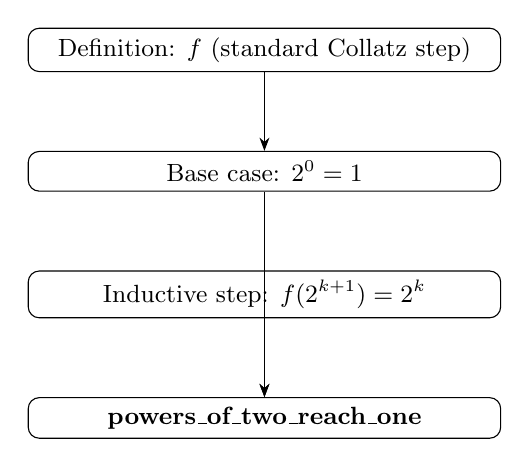
\begin{tikzpicture}[node distance=10mm, every node/.style={font=\small}, box/.style={draw,rounded corners,align=center,minimum width=60mm}, >=Stealth]
\node[box] (defs) {Definition: $f$ (standard Collatz step)};
\node[box, below=of defs] (base) {Base case: $2^0=1$};
\node[box, below=of base] (step) {Inductive step: $f(2^{k+1})=2^k$};
\node[box, below=of step] (main) {\textbf{powers\_of\_two\_reach\_one}};
\draw[->] (defs) -- (base);
\draw[->] (base) -- (main);
\draw[->] (step) -- (main);
\end{tikzpicture}
\end{center}
This is a genuinely flat dependency structure --- a direct contrast to VCE-001's five-lemma chain built on continued-fraction theory.

\section{Formalization}
\begin{table}[h]
\centering
\begin{tabular}{p{6.5cm}p{7cm}}
\toprule
Human mathematics & Lean \\
\midrule
$f(n)=n/2$ (even) or $3n+1$ (odd) & \texttt{def collatzStep (n:N) := if n\%2=0 then n/2 else 3*n+1} \\
$\forall k,\exists m,\ f^{(m)}(2^k)=1$ & \texttt{theorem powers\_of\_two\_reach\_one : forall k, exists m, collatzStep\^{}[m] (2\^{}k) = 1} \\
\bottomrule
\end{tabular}
\caption{Side-by-side comparison, VCE-002.}
\label{tab:sidebyside2}
\end{table}
Table~\ref{tab:sidebyside2}: an exact, direct transliteration --- no representational gap of the kind VCE-001 required (no injectivity bridge needed here). \textbf{Verdict: MATCH.}

\section{Lean Environment}
Lean 4.34.0, Mathlib master \texttt{5ed2965256430c3649e86755f9576b54eca72435}, project \texttt{ico\_collatz\_verification} (this session's own control project, not a third-party repository).

\section{Formal Verification}
\texttt{lake build}: PASS, 8924/8924 jobs, exit 0. No \texttt{sorry}, no \texttt{admit}.

\section{Axiom Audit}
\texttt{propext}, \texttt{Quot.sound}. No \texttt{Classical.choice} --- fully constructive, notably cleaner than VCE-001's headline theorem (which needed classical real-number reasoning for \texttt{Real.logb}).

\section{Independent Check}
\texttt{nanoda\_bin} 0.4.17: \textbf{PASS} --- 1{,}662 declarations, 0 errors, axioms match Gate 6 exactly. This is the gate that stayed open in VCE-001; here it closes cleanly, because this theorem's proof closure is small (pure $\mathbb{N}$ arithmetic) and does not trigger the exporter's large-closure defect.

\section{Computational / Adversarial Tests}
Independent Python brute force, $k \in \{0,\ldots,20,50,100,500,1000\}$: every case reaches $1$ in exactly $k$ steps, matching the proof's prediction exactly. Minimal case ($k=0$) and large-parameter cases ($k=1000$) both covered.

\section{Verification Limitations}
None material for this claim.

\section{Verification Matrix}
\begin{center}
\small
\begin{tabular}{lccccl}
\toprule
Claim & Formal & Axiom & Indep.\ & Comp.\ & Semantic \\
      & Proof  & Audit & Check   & Test   & Match \\
\midrule
\textbf{powers\_of\_two\_reach\_one} & PASS & PASS & \textbf{PASS} & PASS & MATCH \\
\bottomrule
\end{tabular}
\normalsize
\end{center}
Contrast with VCE-001's matrix: every column is PASS here, with no FAIL cell.

\section{Trust / Verification Chain}
\begin{center}
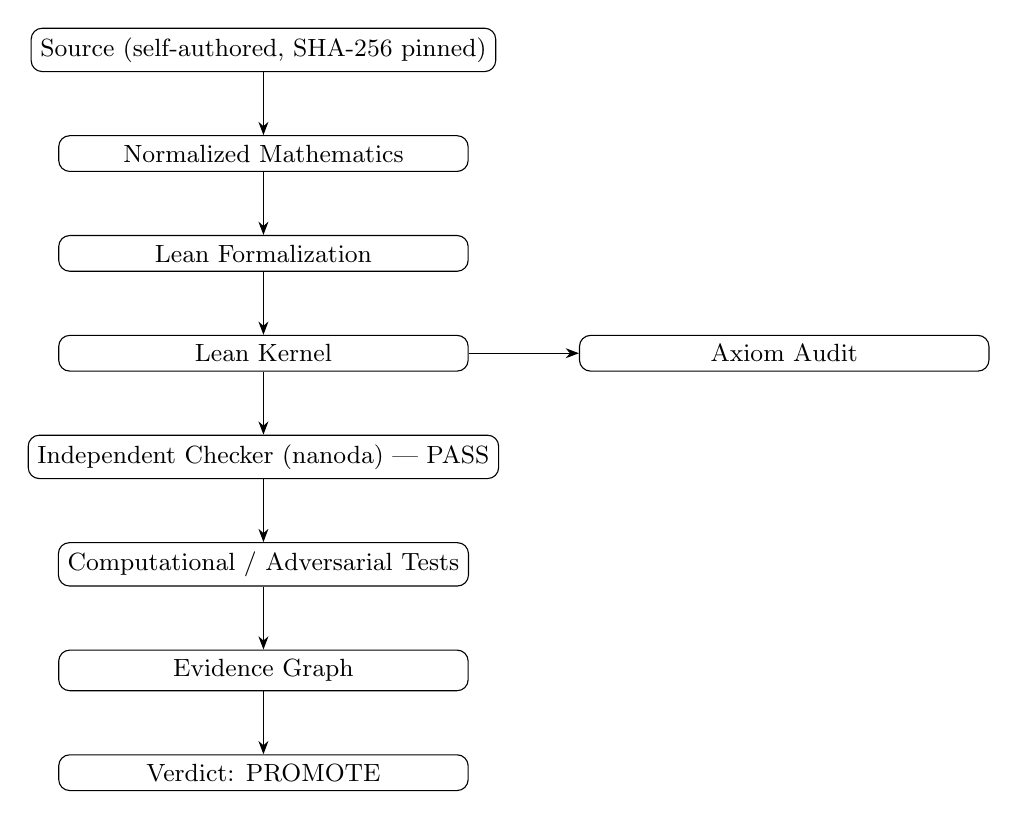
\begin{tikzpicture}[node distance=8mm, every node/.style={font=\small}, box/.style={draw,rounded corners,align=center,minimum width=52mm}, >=Stealth]
\node[box] (source) {Source (self-authored, SHA-256 pinned)};
\node[box, below=of source] (norm) {Normalized Mathematics};
\node[box, below=of norm] (lean) {Lean Formalization};
\node[box, below=of lean] (kernel) {Lean Kernel};
\node[box, below=of kernel] (indep) {Independent Checker (nanoda) --- PASS};
\node[box, below=of indep] (comp) {Computational / Adversarial Tests};
\node[box, below=of comp] (ev) {Evidence Graph};
\node[box, below=of ev] (verdict) {Verdict: PROMOTE};
\node[box, right=14mm of kernel] (axiom) {Axiom Audit};
\draw[->] (source) -- (norm);
\draw[->] (norm) -- (lean);
\draw[->] (lean) -- (kernel);
\draw[->] (kernel) -- (axiom);
\draw[->] (kernel) -- (indep);
\draw[->] (indep) -- (comp);
\draw[->] (comp) -- (ev);
\draw[->] (ev) -- (verdict);
\end{tikzpicture}
\end{center}

\section{Reproducibility Instructions}
\begin{verbatim}
cd ~/ico-collatz/ico_collatz_verification
lake build IcoCollatzVerification.PowersOfTwoReachOne
# expect: Build completed successfully (8924 jobs)
\end{verbatim}
Reproducibility level: \textbf{R4} --- independent verification is itself reproducible, unlike VCE-001.

\section{Correction Ledger}
None for this run. (VCE-001's correction ledger recorded a process-order defect --- Governance Decision was executed before Report Generation, reversed from the canonical order. This run's Report Generation is being executed before its Governance Decision, correcting that.)

\section{Conclusion}
Every trust layer is satisfied for this claim, with no disclosed gap. \textbf{Governance decision: PROMOTE.}

\end{document}
